\section{实现细节}
\subsection{用户管理}
系统支持客户端程序进行用户注册、登录、查询联系人、添加好友等操作。客户端以一定格式向服务器发送请求,服务器端在自己存储的用户状态信息中进行查询,并返回相应的结果。

\subsection{消息收发}
消息收发的过程比较简单,服务器在其中仅仅充当了中转的角色,将来自发送方的消息通过与接收方连接的socket发送给接收方。服务器在用户信息中同时记录
了用户当前的通信状态,例如是否处于聊天模式,与哪位用户进行聊天等等。在客户端,为了实现通信的即时性,分离了接收和发送的功能,交由不同的线程各自
实现。

\subsection{文件收发}
文件收发的过程与消息收发类似,但文件的规模一般较大,无法一次性传输完毕。我采用了分段传输的方法,每次传送一个缓冲区的大小,即2KB。在文件传输开始
之前,会先发送一定格式的消息通知对方即将开始的文件传输过程,这一消息中包含了所要传输的文件大小(字节数),以便接收方判断何时文件接收完毕。经验证
可以成功传输200MB以上大小的文件

\subsection{离线消息、文件收发}
对于离线消息,服务器会将其保存,待收到recvmsg请求后再发送给相应的接收方;对于离线文件,服务器会保存其文件名,并将传输来的文件暂存在本地。收到
收到recvfile请求后,服务器会先发送暂存的文件名,用户指定接收某一文件后才会开始实际的文件传输。

检查时未演示离线消息、文件收发功能,下面提供几张效果截图:

\begin{center}
    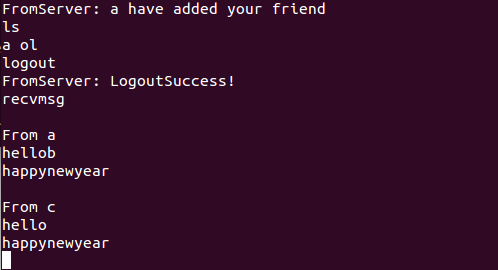
\includegraphics[width=13cm]{image/recvmsg.png}
    \fcaption{recvmsg效果图}
\end{center}

\begin{center}
    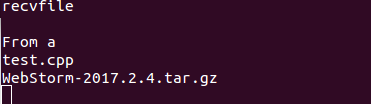
\includegraphics[width=13cm]{image/recvfile.png}
    \fcaption{recvfile效果图}
\end{center}
